\section{引言}
\label{sec:introduction}

长上下文语言模型为文档检索、多跳推理和持久化智能体记忆提供了一种简洁的交互方式：将相关材料放入提示中，并让注意力在需要时将其取回。相应地，模型的上下文窗口已经从数千 token 扩展到数十万 token，而旋转位置嵌入（RoPE）也已成为在这些窗口内编码顺序的标准方法~\citep{su2024roformer}。然而，能够接收长序列并不等同于能够可靠地利用它。长上下文评测反复表明，模型准确率取决于证据出现的位置、其周围无关文本的数量，以及任务所需的检索模式~\citep{liu2024lost,bai2024longbench,hsieh2024ruler}。

本文研究一个更尖锐的矛盾：\emph{证据与查询之间的语义关系可以保持不变，但答案却会随着二者间距的变化而突然改变}。在一个受控的 Qwen3-8B 诊断实验中，两条提示包含相同的金标准规则和相同的末尾问题，区别仅在于第二条提示额外插入了 64 个 filler token。正确首 token 的概率从 42.62\% 降至 1.75\%，其相对于一个格式 token 的 margin 则从 $+1.00$ 变为 $-2.75$。在密集的长度扫描中，这类转变既不平滑，也非永久持续：正确区间与错误区间可能交替出现。仅用单调的“上下文退化”很难解释这一现象。究竟是哪一种内部计算，使语义正确的远程键在特定距离上失去检索优先级？

\begin{figure*}[t]
  \centering
  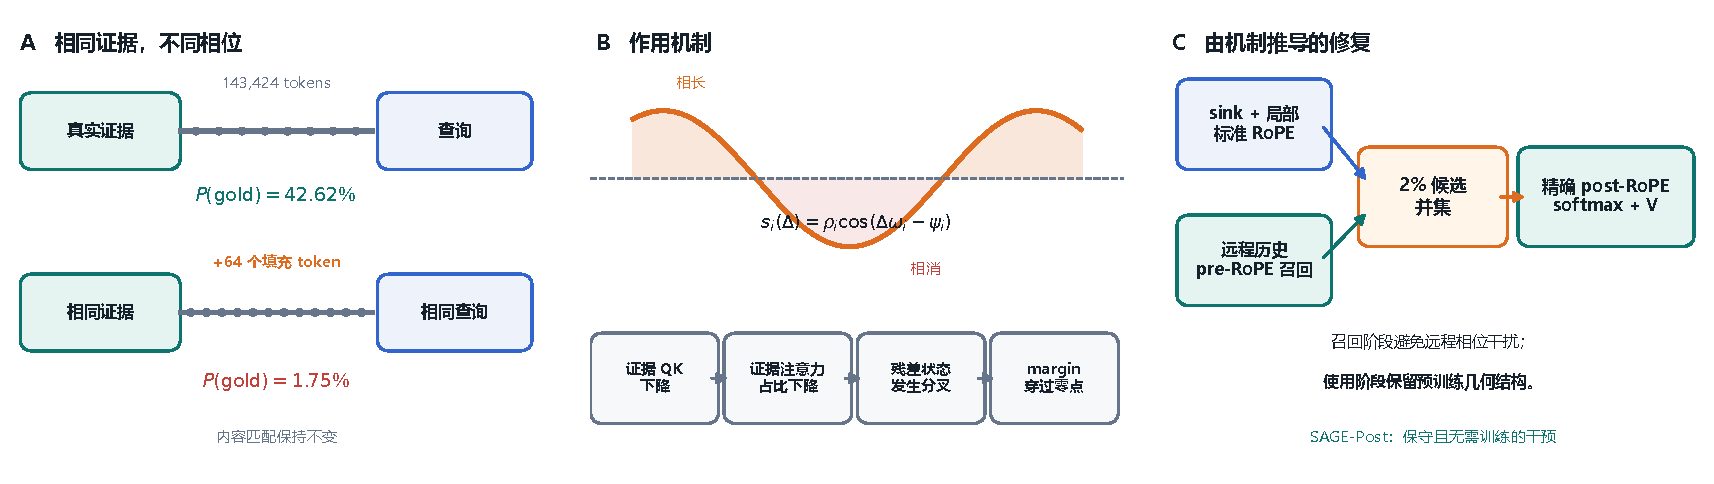
\includegraphics[width=0.98\textwidth]{figures/overview_zh.pdf}
  \caption{本文的“问题—分析—修复”闭环。改变固定证据与查询之间的距离，会在 softmax 之前改变 RoPE 相位。不利相位会抑制金标准 QK 分数，使竞争 token 获得更多概率质量，而改变后的 Value 写入又会导致后续表示发生分叉。\method 修复的正是这一瓶颈：局部 token 保留标准 RoPE，而远程候选先通过无位置信息的语义通道生成，再交由原始 post-RoPE 注意力处理。}
  \label{fig:overview}
\end{figure*}

\textbf{我们定位了 softmax 之前的相位敏感瓶颈。}
RoPE 以不同频率旋转查询/键的每一个二维对。对于固定的 pre-RoPE 内容向量，第 $i$ 个二维对在相对距离 $\Delta$ 下的贡献为
\begin{equation}
  s_i(\Delta)
  = A_i\cos(\Delta\omega_i)+B_i\sin(\Delta\omega_i).
  \label{eq:intro-phase}
\end{equation}
因此，RoPE 将语义兼容性与依赖距离的相位耦合在一起。总分数不一定随距离单调下降，但当高能量频率对发生相消干涉时，相关键可能受到抑制。在 Qwen3-8B 上，将 64 个解析重构的二维对贡献求和，可在四种证据—查询距离下重现测得的第一层分数，最大绝对误差仅为 $1.98\times10^{-3}$。该实验隔离了相位因素：其中的 pre-RoPE 查询和键完全不变。

\textbf{初始分数变化会进一步转化为表示变化。}
Softmax 会将相对分数变化转化为指数级的注意力比例变化。注意力权重的改变会影响写入查询残差流的 Value；因此，后续层并非反复旋转同一个查询，而是从已经发生分叉的隐藏状态中投影出新的 pre-RoPE 查询和键。我们记录了一次 36 层 Qwen3-8B 状态转移中完整的注意力、MLP 和残差向量，并精确重放了每一次 BF16 残差更新。尽管查询嵌入差异为零，第一个注意力分支仍产生了非零残差差异，其范数在最终层达到 312.68。将成功运行的残差状态以因果激活修补的方式注入失败运行的第 16 层，会使输出 margin 从 $-2.75$ 变为 $+0.625$；在第 20 层进行修补，则可将其恢复至 $+1.00$。

\textbf{上述诊断直接决定了修复方法。}
局部顺序对句法和证据内部结构仍然重要，因此全局移除 RoPE 会造成不必要的扰动。反之，若一个远程 token 的内容与查询高度兼容，细粒度距离本身不应将其彻底排除。为此，我们提出 \method（Semantic-Augmented Global Evidence retrieval for RoPE models）。其保守版本 \methodpost 保留 sink token 和近期 token，使用 pre-RoPE QK 提议远程 token，并将 2\% 预算中的剩余部分用于这些候选。随后，该方法取回原始 K/V，并应用模型原有的精确 post-RoPE 分数、softmax 和 Value 聚合。该干预改变的是哪些远程 token 可以参与竞争，而不是所选 token 的评分与使用方式。

\textbf{受控的留出评测支持这一由机制推导出的设计。}
在 8K、16K、32K 和 64K 的每个长度上，我们使用一组固定的、包含 24 个未见两跳实例的数据进行评测。相较于全注意力，\methodpost 将汇总几何均值 \GoldPPL 从 10.851 降至 4.859，并将首 token 准确率从 33.3\% 提高至 47.9\%。在相同预算下，与精确 post-RoPE Top-2\% 选择相比，该方法在 16K 和 32K 上分别将平均 NLL 降低 0.643 和 0.691，对应于 $1.90\times$ 和 $2.00\times$ 的金标准 token 似然比；二者的 95\% 置信区间均不包含零。64K 上的置信区间略微跨过零，且当前实验使用的是合成数据和完整的 pre-RoPE 扫描。因此，本文所主张的是一个受控条件下的机制及其修复方法，而不是普适泛化能力或端到端加速。

本文作出三项贡献。第一，我们形式化了\emph{相位敏感检索失效}：仅由 RoPE 相对相位不同，同一个固定语义匹配就可能获得不同的注意力优先级。第二，我们利用精确有限差分重放和激活修补，将这一第一层效应与注意力总量、残差分叉及最终输出决策联系起来。第三，我们从上述诊断中推导出“局部位置/全局语义”的注意力规则，并通过留出数据、匹配预算的评测验证其价值。
